%-----------------------------------------------------------------------------
% Title, Author, Date
%-----------------------------------------------------------------------------

\title{Modeling dynamic gene expression from RNA-seq time series data using hierarchical Gaussian process-linked negative binomial regression}
\author{
        Spencer Woody\footnote{The University of Texas at Austin, Department of Statistics and Data Science. Data and \textsf{R} script used for this analysis available at \texttt{github.com/spencerwoody/SDS383D/tree/master/FinalProject} } \\
				\texttt{spencer.woody@utexas.edu}
}
\date{\today}

%-----------------------------------------------------------------------------
% Document Class
%-----------------------------------------------------------------------------

\documentclass[11pt]{article}
\usepackage{cite}


%-----------------------------------------------------------------------------
% Packages
%-----------------------------------------------------------------------------

\usepackage{graphicx}
\usepackage{amsmath} 
\usepackage{amssymb}
\usepackage{listings}
\usepackage{enumerate} 


% Theorems, corollaries, lemma
\usepackage{amsthm}
\usepackage[utf8]{inputenc}
\usepackage[english]{babel}
\newtheorem{theorem}{Theorem}[section]
\newtheorem{corollary}{Corollary}[theorem]
\newtheorem{lemma}[theorem]{Lemma}

% Appendix
% \usepackage[toc,page]{appendix}

% Fonts
\usepackage{mathpazo}
\usepackage{avant}
\usepackage{inconsolata}

% Margins
\usepackage[margin=1in]{geometry}

% Define new commands
\usepackage{bm,upgreek}

\newcommand{\tr}{\text{tr}}
\newcommand{\pN}{\mathcal{N}}
\newcommand{\I}{\mathcal{I}}
\newcommand{\R}{\textsf{R} }
\newcommand{\1}{\mathbf{1}}
\newcommand{\0}{\mathbf{0}}
\newcommand{\x}{\mathbf{x}}
\newcommand{\tee}{\mathbf{t}}
\newcommand{\f}{\mathbf{f}}
\newcommand{\K}{\mathbf{K}}
\newcommand{\g}{\mathbf{g}}
\newcommand{\h}{\mathbf{h}}
\newcommand{\y}{\mathbf{y}}
\newcommand{\YY}{\mathbf{Y}}

%-----------------------------------------------------------------------------
% Begin Document -----
%-----------------------------------------------------------------------------


\begin{document}
\maketitle


%-----------------------------------------------------------------------------
%-----------------------------------------------------------------------------
%-----------------------------------------------------------------------------
%---------------------------    START OF TEXT    -----------------------------
%-----------------------------------------------------------------------------
%-----------------------------------------------------------------------------
%-----------------------------------------------------------------------------






%-----------------------------------------------------------------------------
% ABSTRACT
%-----------------------------------------------------------------------------

\begin{abstract}
RNA-seq has emerged as the predominant technology for gene expression analysis. Modeling approaches must take into account the fact that there data are in the form of overdispersed counts. Existing models use the negative binomial distribution. However, there are few existing analysis pipelines which can infer a continuous time course of gene expression. In this paper we present a negative binomial regression model with a logit link on an underlying latent nonparametric time course function taken from a hierarchical Gaussian process to model dynamic gene expression. The advantages of this approach are that it can pool information across replicates and handle the case of samples collected at irregular time intervals. We also present a Gibbs sampler for implementing the model. The model is applied to an RNA-seq time series dataset from an experiment tracking the cellular response of \emph{E. coli} to starvation conditions. We conclude by listing potential extensions of the model and other future work to be done. This paper is written as a final project for the spring 2017 semester course SDS 383D course taught by Professor James Scott at UT-Austin.
\end{abstract}









%-----------------------------------------------------------------------------
% INTRODUCTION
%-----------------------------------------------------------------------------

\section{Introduction}
Recently there has been a proliferation of next-generation sequencing technologies used in bioinformatics. RNA-seq has become the new dominant tool for gene expression analysis, which may be used to infer gene regulatory networks and measure cellular response to external stimuli, to name just a few examples. 

As opposed to microarray data, where gene expression is measured as a continuous variable, RNA-seq data are in the form of counts and are thus discrete. Furthermore, RNA-seq data are often overdispersed (i.e., the variance is larger than the mean), so the Poisson distribution, which has equal variance and mean, is inappropriate to use. Popular analysis pipelines, such as DESeq2 \cite{DESeq2} and edgeR \cite{edgeR}, use the negative binomial distribution. These techniques often fit a generalized linear model (GLM) with some sort of link function, such as the logarithmic link. This may be well suited for tasks such as differential expression between several conditions (e.g. experiment and control), but they are not adept at modeling the continuous time course of gene expression which is likely nonlinear.

In response I propose a negative binomial regression model with a logit link on a latent hierarchical Gaussian process. The motivation for this model comes from \cite{GPmicroarray}, where the authors use a hierarchical Gaussian process to model time series microarray data for samples with multiple replicates. Their approach accounts for hierarchy at the replicate level, but may also be extended to cases like data fusion where an experimenter would also like to pool information across related groups. In our case, we account for the discrete nature of RNA-seq data with the linked negative binomial regression. This allows us to use the same Gaussian process framework in a discrete data context, and the same extensions mentioned in \cite{GPmicroarray} like clustering and data fusion should be applicable to this case too.

% \paragraph{Outline}
% The remainder of this article is organized as follows.
% Section~\ref{Model} gives account of previous work.
% Our new and exciting results are described in Section~\ref{Inference}, Section~\ref{Experiment}, Section~\ref{Conclusion}.
% Finally, Appendix~\ref{mainlemma} gives the conclusions.









%-----------------------------------------------------------------------------
% THE MODEL
%-----------------------------------------------------------------------------

\section{Model}\label{Model}

Let $y_{nrt}$ represent the read count at the time point $t > 0$ for replicate $r \in \left\{ 1, 2, \ldots, R_n \right\}$ of gene $n \in \left\{ 1,2,\ldots N \right\}$. Then $y_{nrt}$ follows a negative-binomial distribution, 
%
%
%
\begin{align*}
	(y_{nrt} | \alpha_{n}, \psi_{nr}(t)) &\sim \text{NB}\left( \alpha_{n} , \frac{\exp\left[ \psi_{nr}(t) \right]}{1 + \exp\left[ \psi_{nr}(t) \right]} \right),
\end{align*}
%
%
%
where $\alpha_n$ is the gene-specific dispersion parameter. For clarity, the parametrization of the negative binomial distribution used in this paper is given in Appendix~\ref{NBdist}. For the sake of this project, I used a plug-in estimate of the dispersion parameter from \cite{DESeq2}, which uses an empirical Bayesian shrinkage estimate of dispersions by pooling across genes with similar mean normalized counts. As for the success probability parameter, there is a logit link on $\psi_{nr}(t),$ a hierarchical Gaussian process described by
%
%
\begin{align*}
	(\psi_{nr}(t) | g_n(t)) &\sim \text{GP}(g_n(t), k_\psi(t, t')) \\
	g_n(t) &\sim \text{GP}(0, k_g(t, t')),
\end{align*}
%
%
%
for some covariance functions $k_\psi(t, t')$ and $k_g(t, t'),$ respectively parameterized by hyperparameters $\theta_\psi$ and $\theta_g$ (which might both be vectors). Notice that the expectation of $y_{nrt}$ is 
%
%
\begin{align}
	\mathbb{E}(y_{nrt} | \alpha_n, \psi_{nr}(t)) &= \alpha_{n} \cdot \exp\left[ \psi_{nr}(t) \right]. \label{expectation}
\end{align} 
%
%
%
We can consider $g_n(t)$ to be the underlying gene-level time course function, and then each $\psi_{nr}(t)$ represents a replicate-level deviation away from this gene-level function.
% 1. hierarchical
% 2. nonparametric
% 3. continuous time
% 4. expected value


%-----------------------------------------------------------------------------
% INFERENCE
%-----------------------------------------------------------------------------

\section{Inference}\label{Inference}

\subsection{Gibbs sampler}

In order to implement the model, we use a data augmentation strategy using the P\'{o}lya-Gamma distribution, originally introduced in \cite{PG} and specifically applied to GLMs for NB regression in \cite{NBregression}, so that we have conditionally conjugate distributions to sample from for the Gibbs sampler. Specifically we introduce a latent $\omega_{nrt}$ corresponding to each $y_{nrt}$ which has the conditional distribution
%
%
%
\begin{align*}
	(\omega_{nrt} | y_{nrt}) &\sim \text{PG}(y_{nrt} + \alpha_{n}, 0).
\end{align*}
%
%
%
The key property of the P\'{o}lya-Gamma distribution which lends itself well for the Gibbs sampler is the expectation 
%
%
%
\begin{align*}
	\mathbb{E}_{\omega_{nrt}}\left[ \exp\left( -\omega_{nrt}\left[ \psi_{nr}(t) \right]^2 / 2 \right) \right] &= \cosh^{-(y_{nrt} + \alpha_{n})}(\psi_{nr}(t) / 2).
\end{align*}
%
%
%
As demonstrated in both \cite{PG} and \cite{NBregression}, the joint likelihood of $y_{nrt}$ given $\omega_{nrt}$ and $\psi_{nr}(t)$ may then be written as
%
%
%
\begin{align*}
	p(y_{nrt} | \psi_{nr}(t), \omega_{nrt}) &\propto \frac{ \left( \exp\left[ \psi_{nr}(t) \right] \right)^{y_{nrt}}}{\left( 1 +  \exp\left[ \psi_{nr}(t) \right] \right)^{\alpha_{n} + y_{nrt}}} \\
	%
	&= \frac{2^{-(y_{nrt} + \alpha_{n})} \cdot \exp\left( \frac{y_{nrt} - \alpha_{n}}{2} \psi_{nr}(t) \right)}{\cosh^{y_{nrt} + \alpha_{n}}(\psi_{nr}(t) / 2)} \\
	%
	&\propto \exp\left( \frac{y_{nrt} - \alpha_{n}}{2} \psi_{nr}(t) \right) \mathbb{E}_{\omega_{nrt}}\left[ \exp\left( -\omega_{nrt}\left[ \psi_{nr}(t) \right]^2 / 2 \right) \right].
\end{align*}
%
%
%
Now suppose we have observations at a vector of times $\mathbf{t}_{nr}$ which has length $T_{nr}$. The data vector of read counts is $\y_{nr} = \left\{ y_{nrt} \right\}_{t\in\mathbf{t}_{nr}}$ which is associated with draws from the GP, $\bm{\uppsi}_{nr} = \left\{ \psi_{nr}(t) \right\}_{t\in\mathbf{t}_{nr}}$. Then there is the latent variable vector $\bm{\upomega}_{nr} = \left\{ \omega_{nrt} \right\}_{t\in\mathbf{t}_{nr}}$. Define the diagonal matrix $\bm{\Omega}_{nr} = \text{diag}\left( \bm{\upomega}_{nr} \right).$ Finally define the vector $\g_n$ be a vector of draws from the GP $g_n(t, t')$ at times $\mathbf{t}_{nr}$ and the matrix $\K_\psi(\mathbf{t}_{nr}, \mathbf{t}_{nr'})$ such that it's $(i, j)$ element is $k_\psi(\mathbf{t}_{nr}[i], \mathbf{t}_{nr'}[j])$ and $\K_g(\mathbf{t}_{nr}, \mathbf{t}_{nr'})$ is defined similarly. Using the definition of the Gaussian process and the properties of the multivariate normal distribution, we can find the marginal prior of distribution of $\bm{\uppsi}_{nr},$  
%
%
%
\begin{align*}
	p(\bm{\uppsi}_{nr} | \g_{n}, \theta_{\psi}) &\sim \pN \left( \f_n, \K_{\psi}(\mathbf{t}_{nr}, \mathbf{t}_{nr}) \right) \\
	%
	%
	p(\f_n | \theta_{g})  &\sim \pN \left( \mathbf{0}, \K_g(\mathbf{t}_{nr}, \mathbf{t}_{nr}) \right) \\
	%
	%
	\Rightarrow p(\bm{\uppsi}_{nr} | \theta_{\psi}, \theta_g) &\sim \pN\left( \mathbf{0}, \K_{\psi}(\mathbf{t}_{nr}, \mathbf{t}_{nr}) + \K_{g}(\mathbf{t}_{nr}, \mathbf{t}_{nr}) \right).
\end{align*}
%
%
%
Let the vector $\bm{\uptheta} = (\theta_\psi, \theta_g)^T$ contain the hyperparameters of both covariance functions, $k_g(t, t')$ and $k_\psi(t, t')$. Now consider the collapsed vector across all replicates. We can write the marginal prior of the concatenated vector $\bm{\uppsi}_n = \left\{ \bm{\uppsi}_{nr} \right\}_{r=1}^{R_{n}}$ as 
%
%
%
\begin{align*}
	p(\bm{\uppsi}_n | \bm{\uptheta}) &= \pN(\mathbf{0}, \K_n)
\end{align*}
%
%
%
where the matrix $\K_n$ is a $R_n \times R_n$ arrangement of matrices, each of which has dimension $T_{nr} \times T_{nr'}$ and is taken as
%
%
%
\begin{align}
	\K_n[r, r'] = \text{cov}(\bm{\uppsi}_{nr}, \bm{\uppsi}_{nr'}) &= \begin{cases}
		\K_g(\mathbf{t}_{nr}, \mathbf{t}_{nr}) + \K_\psi(\mathbf{t}_{nr}, \mathbf{t}_{nr}) & \text{ if } r=r' \\
		\K_g(\mathbf{t}_{nr}, \mathbf{t}_{nr'}) & \text{ otherwise}
	\end{cases}. \label{covmat}
\end{align} 
%
%
%
In plain English, (\ref{covmat}) captures the hierarchical nature of the data; samples from the same gene and same replicate will have covariance coming from both the gene-level and replicate-level functions, $g_n(t)$ and $\psi_{nr}(t),$ while samples from the same gene but different replicates will have covariance only coming from the gene-level function. The conditional posterior of $\bm{\uppsi}_{n}$, given the values of $\bm{\upomega}_{n}$ and the data vector $\y_{n}$ is 
%
%
\begin{align*}
	p(\bm{\uppsi}_{n} | \y_{n}, \bm{\upomega}_{n}, \bm{\uptheta}),  &\propto p(\bm{\uppsi}_n | \bm{\uptheta}) \prod_{r=1}^{R_n} \prod_{t\in\mathbf{t}_{nr}} p(y_{nrt} | \psi_{nr}(t), \omega_{nrt}) \\% p(\y_n | \bm{\uppsi}_n, \bm{\upomega}_n) \\
	%
	%
	 &\propto p(\bm{\uppsi}_n | \bm{\uptheta}) \prod_{r=1}^{R_n} \prod_{t\in\mathbf{t}_{nr}} \exp\left[ -\frac{\omega_{nrt}}{2}\left( \psi_{nr}(t) - \frac{y_{nrt} - \alpha_{n}}{2 \omega_{nrt}} \right)^2 \right] \text{, define } z_{nrt} = \frac{y_{nrt} - \alpha_{n}}{2 }, \\
	%
	%
	&\propto p(\bm{\uppsi}_{n} | \bm{\uptheta}) \cdot \exp \left[ -\frac{1}{2} \left( \bm{\uppsi}_{n} - \bm{\Omega}^{-1}_{n} \mathbf{z}_n \right)^T \bm{\Omega}_{n} \left( \bm{\uppsi}_{n} - \bm{\Omega}_{n}^{-1} \mathbf{z}_n \right) \right] \\
	%
	%
	&\propto \pN \left(\bm{\uppsi}_{n} | \bm{\Sigma}_{n} \mathbf{z}_n, \bm{\Sigma}_{n}  \right), \text{ with } \bm{\Sigma}_{n} = \left( \K_n^{-1} + \bm{\Omega}_{n} \right)^{-1}.
\end{align*}
%
%
%
%
The conditional posterior of each $\omega_{nrt}$ is 
%
%
%
\begin{align*}
	p(\omega_{nrt} | y_{nrt}, \psi_{nr}(t)) &\propto \left[ \exp\left( -\omega_{nrt}\left[ \psi_{nr}(t) \right]^2 / 2 \right) \right] \cdot \text{PG}(\omega_{nrt} | y_{nrt} + \alpha_{n}, 0) \\
	&\propto \text{PG}(\omega_{nrt} | y_{nrt} + \alpha_{n}, \psi_{nr}(t)).
\end{align*}
%
%
%
Therefore the Gibbs sampler involves iteratively sampling from 
%
%
%
\begin{align}
	 (\bm{\uppsi}_{n} | \y_{n}, \bm{\upomega}_{n}, \bm{\uptheta}) &\sim \pN \left(\bm{\uppsi}_{n} | \bm{\Sigma}_{n} \mathbf{z}_n, \bm{\Sigma}_{n}  \right), \text{ with } \bm{\Sigma}_{n} = \left( \K_n^{-1} + \bm{\Omega}_{n} \right)^{-1} \\
	(\omega_{nrt} | y_{nrt}, \psi_{nr}(t)) &\sim \text{PG}(\omega_{nrt} | y_{nrt} + \alpha_{n}, \psi_{nr}(t)).
\end{align}
%
%
%
\subsection{Prediction of gene- and replicate-level time course}
%
%
%
At each iteration of the Gibbs sampler, we can also sample from the marginal posterior distribution of the underlying gene- and replicate-level time series functions. That is to say, we sample $\mathbf{g}_n^\star$ which is a series of draws from $g_n(t)$ at ``new'' times $\mathbf{t}_{n}^\star$, and we also sample $\bm{\uppsi}_{nr}^{\star}$ which is $\psi_{nr}(t)$ at ``new'' times $\mathbf{t}_{nr}^\star$ for each $r$. The respective joint distributions between these vectors and $\bm{\uppsi}_{n}$ are 
%
%
\begin{align*}
	\begin{bmatrix}
			\bm{\uppsi}_{n} \\
			\mathbf{g}_{n}^\star 
	\end{bmatrix} &\sim \pN \left( \mathbf{0}, \begin{bmatrix}
 			\K_n & \K_{n\star}^T \\
 			\K_{n\star} & \K_{n\star\star}
 		\end{bmatrix} \right) \\
%
%
	\begin{bmatrix}
		\bm{\uppsi}_{n} \\
		\bm{\uppsi}_{nr}^\star
	\end{bmatrix} &\sim \pN \left( \mathbf{0}, \begin{bmatrix}
		\K_n & \K_{nr\star}^T \\
		\K_{nr\star} & \K_{nr\star\star}
	\end{bmatrix} \right) 
\end{align*}
%
%
with $\K_{n\star}$ and $\K_{nr\star}$ are defined element-wise such that 
%
%
\begin{align*}
	\K_{n\star}[i, j] &= \text{cov}\left( \mathbf{g}_{n}^\star[i] , \bm{\uppsi}_{n}[j] \right) = k_g(\mathbf{t}_{n}^\star[i], \mathbf{t}_n[j]) \\
	%
	%
	\K_{nr\star}[i, j] &= \text{cov}\left( \bm{\uppsi}_{nr}^\star[i], \bm{\uppsi}_{n}[j] \in \bm{\uppsi}_{nr'}  \right) = \begin{cases}
		k_g(\mathbf{t}_{nr}^\star[i], \mathbf{t}_n[j]) + k_\psi(\mathbf{t}_{nr}^\star[i], \mathbf{t}_n[j]) & \text{if } r = r' \\
		k_g(\mathbf{t}_{nr}^\star[i], \mathbf{t}_n[j]) & \text{otherwise}
	\end{cases},
\end{align*}
%
%
and the matrices $\K_{n\star\star}$ and $\K_{nr\star\star}$ are
%
%
\begin{align*}
	\K_{n\star\star} &= \K_g(\mathbf{t}_{n}^\star, \mathbf{t}_{n}^\star) \\
	\K_{nr\star\star} &= \K_g(\mathbf{t}_{nr}^\star, \mathbf{t}_{nr}^\star) + \K_\psi(\mathbf{t}_{nr}^\star, \mathbf{t}_{nr}^\star). 
\end{align*}
%
%
%
The conditional distribution of $\mathbf{g}_n^\star$ given $\bm{\uppsi}_{n}$ is 
%
%
\begin{align*}
	(\mathbf{g}_{n}^\star | \bm{\uppsi}_{n} , \bm{\uptheta}) \sim \pN\left( \K_{n\star}\K_n^{-1}\bm{\uppsi}_{n},\; \K_{n\star\star} - \K_{n\star}\K_n^{-1}\K_{n\star}^T \right).
\end{align*}
%
%
%
Given the fact that the marginal posterior of $\bm{\uppsi}_{n}$ is
%
%
\begin{align*}
	(\bm{\uppsi}_{n} | \y_{n}, \bm{\upomega}_{n}, \bm{\uptheta})  &\sim \pN \left(\bm{\Sigma}_{n} \mathbf{z}_n, \bm{\Sigma}_{n}  \right),
\end{align*}
%
%
and using Lemma \ref{lem:joint} we can write the marginal posterior of $\mathbf{g}_n^\star$ as 
%
%
\begin{align}
	(\mathbf{g}_n^\star | \y_{n}, \bm{\upomega}_{n}, \bm{\uptheta}) &\sim \pN \left( \K_{n\star}\K_n^{-1}\bm{\Sigma}_{n} \mathbf{z}_n,\; \K_{n\star}\K_n^{-1}\bm{\Sigma}_{n}\K_n^{-1} \K_{n\star}^T + \K_{n\star\star} - \K_{n\star}\K_n^{-1}\K_{n\star}^T \right). \label{infer_gene}
\end{align}
%
%
Similarly, the marginal posterior of $\bm{\uppsi}_{nr}^{\star}$ is 
%
%
\begin{align}
	(\bm{\uppsi}_{nr}^{\star} | \y_{n}, \bm{\upomega}_{n}, \bm{\uptheta}) &\sim \pN \left( \K_{nr\star}\K_n^{-1}\bm{\Sigma}_{n} \mathbf{z}_n,\; \K_{nr\star}\K_n^{-1}\bm{\Sigma}_{n}\K_n^{-1} \K_{nr\star}^T + \K_{nr\star\star} - \K_{nr\star}\K_n^{-1}\K_{nr\star}^T \right). \label{infer_rep}
\end{align}
%
%
%
Using our Gibbs sampler framework, at each iteration we store draws from (\ref{infer_gene}) and (\ref{infer_rep}). Then we can make a 95\% posterior credible band by taking the 2.5\% and 97.5\% quantiles for the time series at each time in $\mathbf{t}_{n}^\star$ and $\mathbf{t}_{nr}^\star$.
%
%
%
\subsection{Choice of covariance function and hyperparameters}
%
%
%
For this analysis I chose the $\text{Mat\'{e}rn(5/2)}$ covariance function for both GPs,
%
%
\begin{align*}
	k_g(t, t') &= \tau_g^2 \exp\left\{ 1 + \sqrt{5} \cdot \frac{d}{b_g} + \frac{5}{3} \cdot \frac{d^2}{b_g^2} \right\} \exp \left\{ -\sqrt{5} \cdot \frac{d}{b_g} \right \} , \; d = \|t - t' \|, \\
	k_\psi(t, t') &= \tau_\psi^2 \exp\left\{ 1 + \sqrt{5} \cdot \frac{d}{b_\psi} + \frac{5}{3} \cdot \frac{d^2}{b_\psi^2} \right\} \exp \left\{ -\sqrt{5} \cdot \frac{d}{b_\psi} \right \} , \; d = \|t - t' \|,
\end{align*}
%
%
so, for the gene-level covariance function the hyperparameters are $\theta_g = (b_g, \tau_g^2)^T$, and we refer to $b_g$ as the \emph{relative length} parameter and $\tau_g^2$ is the \emph{amplitude} parameter. For the replicate-level covariance function, the hyperparameters are $\theta_\psi = (b_\psi, \tau_\psi^2)^T$. Of course, inferences made from Gaussian processes are highly sensitive to the hyperparameters contained within the covariance function. It is common to use plug-in estimates from type-II marginal likelihood maximization, i.e.
%
%
%
\begin{align}
	\hat{\bm{\uptheta}} = \arg \max_{\bm{\uptheta}} p(\y_n | \bm{\uptheta}) = \arg \max_{\bm{\uptheta}} \int p(\y_n | \bm{\uppsi}_n, \bm{\uptheta}) p(\bm{\uppsi}_n| \bm{\uptheta}) d \bm{\uppsi}_n \label{type2}
\end{align}
%
%
%
However, in this case there is no closed form solution to the marginal likelihood function in (\ref{type2}) so this is difficult to do in practice. It might also be preferable to integrate over uncertainty of the hyperparameters, in which case we set the hyperprior $p(\bm{\uptheta})$ and then at each iteration of the Gibbs, sample from the density
%
%
%
\begin{align*}
	p( \bm{\uptheta} | \y_{n}, \bm{\upomega}_{n}, \bm{\uppsi}_{n}) &\propto p(\bm{\uppsi}_{n} | \y_{n}, \bm{\upomega}_{n}, \bm{\uptheta}) \cdot p(\bm{\uptheta}).
\end{align*}
%
%
%
This presents another issue because we must choose an appropriate hyperprior, which is likely not conjugate to $p(\bm{\uppsi}_{n} | \y_{n}, \bm{\upomega}_{n}, \bm{\uptheta})$, so then we need to perform a Metropolis-Hastings step at each iteration. 

%-----------------------------------------------------------------------------
% EXPERIMENT
%-----------------------------------------------------------------------------

\section{Experiment}\label{Experiment}

We implemented our model on an RNA-seq dataset from an experiment in \cite{Houser}, where the authors collected samples from \emph{Escherichia coli} to track cellular response to starvation conditions at nine irregularly spaced time-points: 3, 4, 5, 6, 8, 24, 48, 168, and 336 hours. For this analysis we estimated on a logarithmic time scale to put the times on a more dense space. We coded the Gibbs sampler in \textsf{R} as derived above and used the \texttt{BayesLogit} package \cite{PG} to sample from the P\'{o}lya-Gamma distribution.

As mentioned earlier, the choice of hyperparameters is critical because they are highly influential on the outcome of our results. Our first idea was to implement a Metropolis-Hastings step to sample the hyperparameters at each Gibbs iteration. Before doing this, we tried using an estimate of the hyperparamters found by maximizing the log-likelihood of $p(\bm{\uppsi}_{n} | \y_{n}, \bm{\upomega}_{n}, \bm{\uptheta})$ with respect to $\bm{\uptheta}$ using the output of $\bm{\uppsi}_n$ from the Gibbs sampler (which is equivalent to using a MAP estimate with a flat hyperprior), using the \texttt{optim} command in \textsf{R}. However, with this approach we found that this optimization method gave wildly varying results, with each estimated hyperparameter ranging across multiple orders of magnitude. This may suggest that the log-likelihood function is very flat, so it is difficult to find a global maximum, which in turn highlights a need to have an appropriate hyperprior. Due to a shortage in available time, for the purposes of this project, the hyperparameters were somewhat arbitrarily set to $b_g = b_\psi = 2$ and $\tau_g = \tau_\psi = 1$ 

Figure \ref{fig:grids} shows the results of the model implemented on the dataset. There were 4000 Gibbs iterations after a burn-in of 1000 iterations. Each row of the figure represents one gene. The ribbon on each plot is the 95\% posterior credible band for the function, and the solid black line is the posterior median. The left panel of each row shows the infered gene-level time course function, and the right panel shows each infered replicate-level time course function. On the replicate panels, there is also overlaid data, with each datapoint normalized by the transormation $\log(y_{nrt} / \alpha_n)$, derived from \ref{expectation}, so that the data and the time course function are on the same scale. Some read counts are equal to zero and the logarithmic function is not defined at zero, so these counts are shown with semi-circles along the bottom of the plots. The results show that the model fits the data well, and we are able to estimate a sensible gene-level function in each case. We should not expect the fitted curves to pass through or nearly through all the data because the time course function is related to the \emph{expected} read count for a given time.

\begin{figure}[htp!]
	\centering
		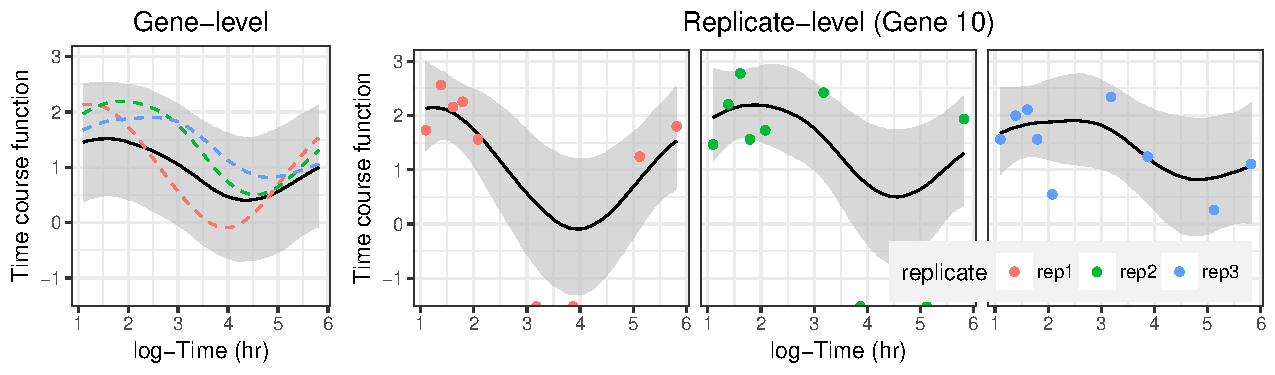
\includegraphics[scale=0.8]{img/grid_gene10.pdf}
		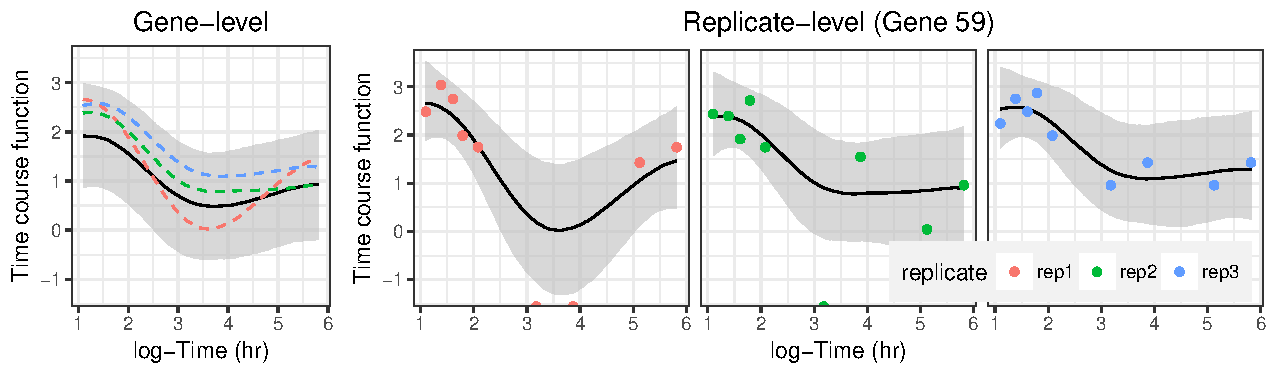
\includegraphics[scale=0.8]{img/grid_gene59.pdf}
		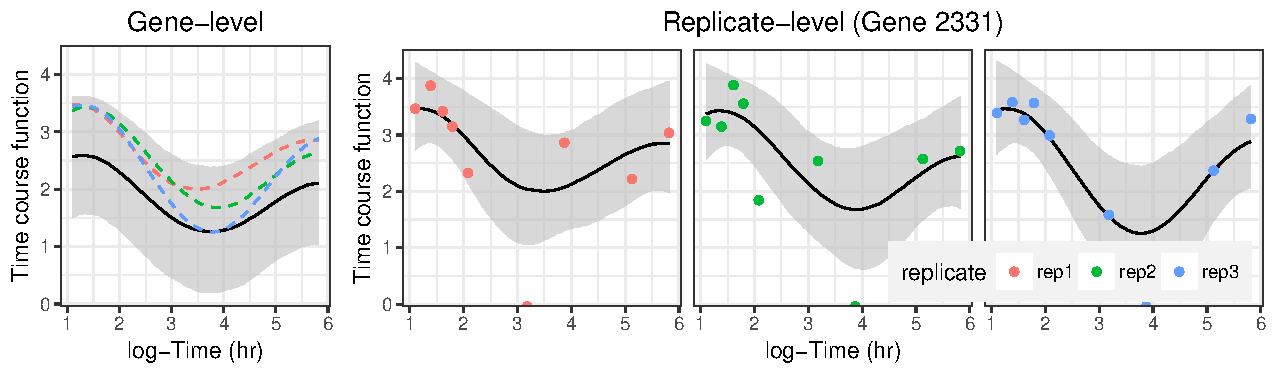
\includegraphics[scale=0.8]{img/grid_gene2331.pdf}
		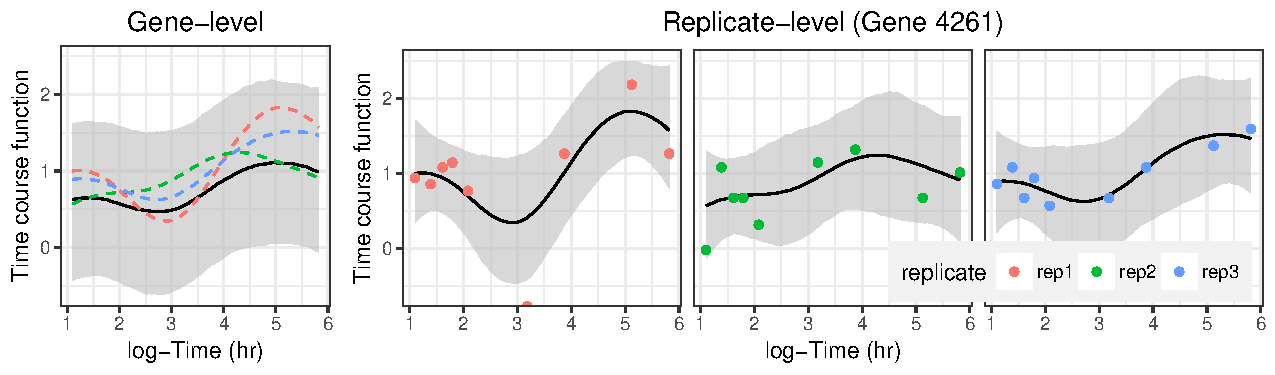
\includegraphics[scale=0.8]{img/grid_gene4261.pdf}
	\caption{Gene- and replicate-level time series functions for selected genes with overlaid normalized data}
	\label{fig:grids}
\end{figure}




%-----------------------------------------------------------------------------
% CONCLUSTION
%-----------------------------------------------------------------------------

\section{Conclusion}\label{Conclusion}

In this report we were mostly successful in applying to RNA-seq data our negative binomial regression model with a logit-linked nonparametric time course function from a Gaussian process. The Gibbs sampler for making inference is presented, and then implemented in \textsf{R}. However, there remain problems with tuning the hyperparameters of the Gaussian processes, and this issue should be addressed because picking the right hyperparameters is essential to deriving meaningful results. Similar to what is explained in \cite{GPmicroarray}, there are several extensions of this model which are worth exploring. For instance, it is possible to generalize to different levels of hierarchy, such as data from different experiments. Clustering genes based on similar expression time dynamics can be used for inferring gene regulatory networks or gauging global cellular response qualitatively through gene ontology. Differential expression analysis, a vital method in transcriptomics, is explored in context of Gaussian processes applied to microarray data in \cite{GPDE}, and this should also be extended to the model presented here.






%-----------------------------------------------------------------------------
% REFERENCES
%-----------------------------------------------------------------------------


\bibliography{FinalProject.bib}{}
\bibliographystyle{unsrt}
% \bibliography{FinalProject.bib}
% \bibliography{simple}












%-----------------------------------------------------------------------------
%-----------------------------------------------------------------------------
%-----------------------------------------------------------------------------
% APPENDIX / APPENDICES
%-----------------------------------------------------------------------------
%-----------------------------------------------------------------------------
%-----------------------------------------------------------------------------

% \pagebreak

\appendix

%-----------------------------------------------------------------------------
% PARAMETERIZATION OF NB DISTRIBUTION
%-----------------------------------------------------------------------------

\section{Parameterization of Negative Binomial distribution}\label{NBdist}

Let $Y$ be a negative binomial-distributed random variable which has support over the nonnegative integers with \emph{dispersion} parameter $r \in {(0,\infty)}$, and \emph{success probability} parameter $p \in (0, 1)$. This may be denoted as 
%
%
\begin{align*}
	Y \sim \text{NB}(r, p),
\end{align*}
%
%
and $Y$ has the probability mass function
%
%
\begin{align*}
	\Pr(Y = k) &= \frac{\Gamma(r + k)}{k! \Gamma(r)} \cdot (1-p)^{r} p^{k} \\
	&= \binom{k + r - 1}{k} \cdot (1-p)^{r} p^{k} \;\text{  if  }\; r\in \left\{ 1, 2, \ldots \right\}.
\end{align*}
%
%
The mean and variance of $Y$ are, respectively,
%
%
\begin{align*}
	\mathbb{E}(Y) &\equiv \mu = \frac{p}{1-p} \cdot r \\
	\text{Var}(Y) &= \frac{p}{(1-p)^2} \cdot r = \mu + \mu^2 / r.
\end{align*}
%
%
Note that $\text{Var}(Y) > \mathbb{E}(Y),$ which encapsulates the \emph{overdispersion} property of the negative binomial distribution, as opposed to the Poisson distribution which has equal mean and variance. When $r$ is a positive integer, we may interpret $Y$ as the number of successes before the $r$th failure in a series of independent Bernoulli trials with succeess probability $p$. 

%-----------------------------------------------------------------------------
% MAIN LEMMA 
%-----------------------------------------------------------------------------

\section{Lemma}\label{mainlemma}

\begin{lemma}\label{lem:joint}
	Define the random vectors $x$ and $\gamma$ such that the conditional distribution of $x$ given $\gamma$ and the marginal distribution of $\gamma$ are, respectively,
	%
	% 
	\begin{align*}
		(x | \gamma) &\sim \pN_n(A\gamma, \Sigma) \\
		\gamma &\sim \pN_p(m, V),
	\end{align*}
	%
	%
	where $A$ is a $n \times p$ matrix. Then the joint distribution of $(x, \gamma)^T$ is 
	%
	%
	\begin{align}
		\begin{bmatrix}
			x \\
			\gamma
		\end{bmatrix} &\sim \pN \left( \begin{bmatrix}
			Am \\
			m
		\end{bmatrix}, \begin{bmatrix}
			AVA^T + \Sigma & AV \\
			VA^T & \Sigma
		\end{bmatrix} \right). \label{eqn:lemmaresult}
	\end{align}
	%
	%
	\begin{proof}
		Equivalently, $x$ may be written as  
		%
		%
		\begin{align*}
			x = A\gamma + \eta,\; \eta &\sim \pN_n(0, \Sigma) 
		\end{align*}
		%
		%
		and then $(x, \gamma)^T$ is multivariate normal because it can be written as an affine transformation of independent multivariate normal variables,
		%
		%
		\begin{align*}
			\begin{bmatrix}
				x \\
				\gamma
			\end{bmatrix} &= \begin{bmatrix}
				A \\ 
				\mathcal{I}_p
			\end{bmatrix} \gamma + \begin{bmatrix}
				\mathcal{I}_n \\
				\mathcal{O}_{p \times n}
			\end{bmatrix} \eta.
		\end{align*}
		%
		%
		From this, the mean and covariance matrix in (\ref{eqn:lemmaresult}) may be derived from properties of the multivatiate normal distribution.
	\end{proof}
\end{lemma} 


%-----------------------------------------------------------------------------
%-----------------------------------------------------------------------------
%-----------------------------------------------------------------------------
%-----------------------------------------------------------------------------
%-----------------------------------------------------------------------------
%-----------------------------------------------------------------------------
%-----------------------------------------------------------------------------
% END
%-----------------------------------------------------------------------------
%-----------------------------------------------------------------------------
%-----------------------------------------------------------------------------
%-----------------------------------------------------------------------------
%-----------------------------------------------------------------------------
%-----------------------------------------------------------------------------
%-----------------------------------------------------------------------------

\end{document}


